\documentclass{article}

\usepackage[landscape]{geometry}
\usepackage{tikz}
\usepackage[utf8]{inputenc}

%\usetikzlibrary{shapes, geometric, arrows}

\tikzstyle{process} = [rectangle, minimum width = 1.5cm, minimum height = 1cm, 
	text centered, ultra thick, draw = black]
\tikzstyle{arrow} = [ultra thick, ->]	

\begin{document}
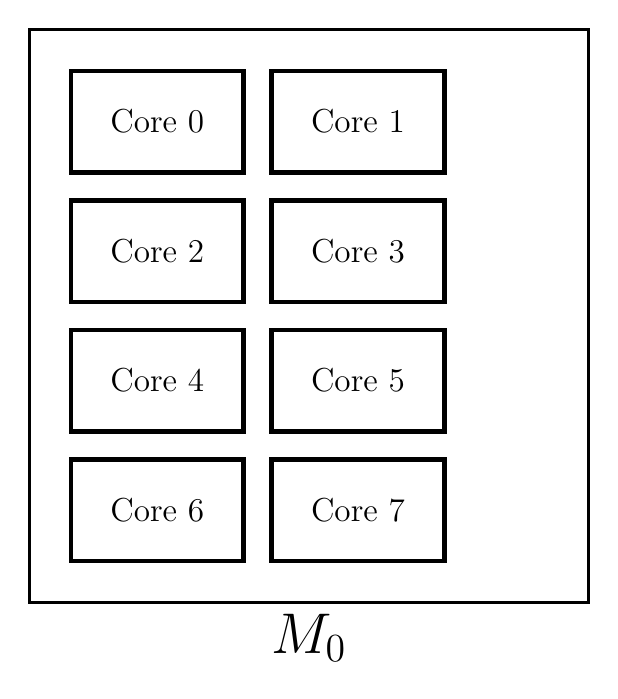
\begin{tikzpicture}[node distance = 8cm]

\node [matrix, draw = black, very thick, 
	inner sep = 5mm, row sep = 3mm, column sep = 3mm, 
	label = below:\huge $M_0$]
{
	\node (server0) [process] {\large Core 0}; & 
	\node (server1) [process] {\large Core 1}; &
	[1cm]\\

	\node (server2) [process] {\large Core 2}; & 
	\node (server3) [process] {\large Core 3}; &
	[1cm]\\

	\node (server4) [process] {\large Core 4}; & 
	\node (server5) [process] {\large Core 5}; &
	[1cm]\\

	\node (server6) [process] {\large Core 6}; & 
	\node (server7) [process] {\large Core 7}; &
	[1cm]\\
};


\end{tikzpicture}
\end{document}
